% !TEX encoding = UTF-8 Unicode
% !TEX TS-program = xelatex

%\documentclass[draftcls,conference]{IEEEtran}
\documentclass[conference]{IEEEtran}
\IEEEoverridecommandlockouts
%\overrideIEEEmargins
% See the \addtolength command later in the file to balance the column lengths
% on the last page of the document

\usepackage{indentfirst}
\usepackage[colorlinks=true,citecolor=red]{hyperref}
                         
\usepackage{amsmath} % assumes amsmath package installed
\usepackage{amssymb}  % assumes amsmath package installed
\usepackage{amsfonts}
\usepackage{amsthm}
\usepackage{pstricks}
\usepackage{fontspec, xunicode, xltxtra}
\usepackage{subfigure}
\usepackage{listings}
\lstset{
    frameround=fttf,
    basicstyle=\ttfamily,
    columns=flexible ,
    breaklines=true,       
    numbers=left,                                        % 在左侧显示行号
    frame=lines,                                          % 显示背景边框,不显示=none
    framextopmargin=1pt,
    captionpos=b,
    %backgroundcolor=\color[RGB]{245,245,244},            % 设定背景颜色
    keywordstyle=\color[RGB]{40,40,255},                 % 设定关键字颜色
    numberstyle=\footnotesize\color{darkgray},           		 % 设定行号格式
    numbersep=3pt,  									%设置行号与代码的距离,默认是5pt
    commentstyle=\it\color[RGB]{0,96,96},                % 设置代码注释的格式
    stringstyle=\rmfamily\slshape\color[RGB]{128,0,0},   % 设置字符串格式
    showstringspaces=false,                              % 不显示字符串中的空格
    %language=c,                                        % 设置语言
    %morekeywords={Import, from, Operator, Apply, End, def, =, ==, then,},
    %emph={source, target, ObjCombine, PortAllocate, },
    %emphstyle=\color{Violet}, 
    morecomment=[l]{--},							%添加注释
}



%\def \qed {\hfill \vrule height6pt width 6pt depth 0pt} %产生证明结束的方块

\theoremstyle{definition}
\newcounter{defncounter}
\setcounter{defncounter}{2}
\newtheorem{defn}{Definition}[defncounter]

%\setlength{\parindent}{1.5em}
\title{\LARGE \bf
Collaborative design: Explore CPSs analysis capabilities of SysML-based tools with AADL and Hybrid Annex
}

%\author{ \parbox{3 in}{\centering Huibert Kwakernaak*
%         \thanks{*Use the $\backslash$thanks command to put information here}\\
%         Faculty of Electrical Engineering, Mathematics and Computer Science\\
%         University of Twente\\
%         7500 AE Enschede, The Netherlands\\
%         {\tt\small h.kwakernaak@autsubmit.com}}
%         \hspace*{ 0.5 in}
%         \parbox{3 in}{ \centering Pradeep Misra**
%         \thanks{**The footnote marks may be inserted manually}\\
%        Department of Electrical Engineering \\
%         Wright State University\\
%         Dayton, OH 45435, USA\\
%         {\tt\small pmisra@cs.wright.edu}}
%}

%\author{Hui ZHAO, TengFei LI}
%\author{\IEEEauthorblockN{Hui Zhao}
%\IEEEauthorblockA{Universit\'e C\^ote d'Azur, I3S, INRIA\\
%hui.zhao@inria.fr}%2004 Route des Lucioles,Valbonne, 06902, France\\

%\and
%\IEEEauthorblockN{Fr\'ed\'eric Mallet}
%\IEEEauthorblockA{Universit\'e C\^ote d'Azur, I3S, INRIA, UMR 7271 CNRS\\
%frederic.mallet@inria.fr}
%\and
%\IEEEauthorblockN{Ludovic Apvrille}
%\IEEEauthorblockA{LTCI, Telecom ParisTech, Universit\'e Paris Saclay.\\
%ludovic.apvrille@telecom-paristech.fr}
%\thanks{This work was financially Supported by the CLARITY project and by a UCN@Sophia Labex scholarship.}}

\begin{document}
%\watermark{60}{10}{DRAFT}%水印


\maketitle
\thispagestyle{empty}
\pagestyle{empty}


%%%%%%%%%%%%%%%%%%%%%%%%%%%%%%%%%%%%%%%%%%%%%%%%%%%%%%%%%%%%%%%%%%%%%%%%%%%%%%%%
\begin{abstract}
The design of Cyber-Physical Systems (CPSs) has become increasingly complex and challenging. The collaborative design is a potential approach to deal with the rise of the complexity of system design which attracts more and more attention. Collaborative design relied on Model-driven engineering (MDE) involving several modeling languages (such as SysML, AADL, etc.) and using principles of separation of concerns as well as domain-specific languages (DSL). It makes stakeholders from diverse domains to work in a coordinated manner on different aspects of the system. It could help in reducing the gap between heterogeneous domains and making diverse expertise work together to produce a coherent and complete system. Therefore, there are requirements for the collaborative design to allow different domain experts to work together. In this paper, we show how to use the coordinated metamodel approach in MDE as a systematic way to gather isolated domain models and cross-cutting concerns. In practice, we proposed a set of transformation operators to manipulating metamodels; it aims to enrich the capacities of the platform by blending different languages seamlessly, as well as perform verification and validation respectively at the high-level and early stage of development. We illustrate our approach through experiments in the train traction controlling system design process.
\end{abstract} 

\section{introduction}\label{sec:intro}
The design of Cyber-Physical Systems (CPSs) has become increasingly complex and challenging. The developer should face numerous aspects, and each aspect has their problem space and characteristics. 

As the Model-Based Engineering (MBE) has emerged as a key set of technologies to engineer the complex system. Experts thus usually used models and metamodels as the common countermeasure to capturing and solving the problems. In recent years, a number of modeling languages target CPSs have been standardized, but, to the best of our knowledge, none of them provide the full range required to deal effectively with the kinds of CPSs's complex that we have encountered. Some of them, such as Systems Modeling Language (SysML)~\cite{Group:2017vva}, a more general-purpose language, focus on the “big picture” requirements, functional and architectural views, whereas others, such as Architecture Analysis and Design Language (AADL)~\cite{Anonymous:aEmc45af} address the more detailed platform-oriented and physical aspects of such systems.  

Since Cyber-Physical Systems interact with surrounding physical environment frequently, and discrete, continuous and hybrid behaviors describe the physical part, fox example, the physical symptom used DEs or PDEs (Partial Differential Equations) to express. A more general case is the hybrid system which is the continuous dynamics of interactions between a control system and its environment, thus Ahmad et al~\cite{Ahmad:2014:HAA:2692956.2663178} proposed a hybrid annex of AADL to intensify AADL's capability to describe hybrid systems. In this paper, we also considered HA (hybrid annex) as a part of the target model. 

Although AADL was a sophisticated analysis language and existing IDE tools such as OSATE~\cite{osate2ref} which can describe and verify both functional and non-functional properties of AADL models, it still insufficient to cater comprehensive system design and the need of abilities for engineering~\cite{behjati2011extending}. Therefore, AADL must be used with the upstream modeling language such as SysML and supporting engineering environment like  Capella/Arcadia~\cite{capella2014}\cite{AModelBasedEngine:JlLHIqkz}. 

Capella platform and its method ARCADIA (\textbf{ARC}hitecture \textbf{A}nalysis and \textbf{D}esign \textbf{I}ntegrated \textbf{A}pproach) are to some extent a SysML-like solution to design the architecture of complex systems using models. However, unlike SysML, it appears to be a domain-specific language (DSL) which was preferred in order to ease appropriation by all stakeholders, usually not familiar with general-purpose, generic languages such as UML or SysML. Rather than having modeling “experts” owning the model on behalf of systems engineers, the ultimate goal of Arcadia is to have systems engineers pay more attention to global system design. 

It is seldom the case that one development platform or single language can adapt to all aspects with assumption one-size-fits-all. Due to the engineers involved various modeling languages to different model domains respectively, and the engineers who from the different domain, each one has domain-specific tools. It does not only result in the proliferation of languages and its extensions for describing a variety of CPSs's aspects but also make the design complexity of CPSs increase. Meanwhile, the gaps between languages and platforms brought additional problems such as coherent and consistent problems, which is exposed at integration and simulation stages and further augment the complexity, make it skyrocketing. 
 
To reduce the gaps and eliminate inconsistencies between SymML--like tool Capella/Arcadia and architecture design language AADL and its hybrid annex (HA), also to benefit from both of their powerful capabilities and strong points, we present a suite of evolving combining approach. In despite of existing a lot of studies on the combining SysML and AADL~\cite{de2012combining} or on the extending SysML with AADL~\cite{behjati2011extending}. Differ from above studies; our method dedicates to smoothly combine engineering platform Capella/Arcadia, AADL and its annex, in this way, one could design global system at a high level and then seamlessly refine the models within AADL and its annex. That can also properly extend Arcadia's capability, and make it can perform analysis of discrete behavior variation and continuous environmental domain.    


This paper presents an approach was to characterize the discrete and continuous properties of CPSs by models and abstract metamodels, respectively. Then merge the two metamodels to generate new metamodel at high abstract level. The engineer can use this generated metamodel to create kaleidoscopic instance models which can be used to further analysis (e.g., timing, safety). In this way,  it allows the original engineering platform is capable of scaling to a wider range of capabilities through the use of relevant languages. Compared with similar studies, our approach makes \textbf{\textit{three following major contributions}}:

\begin{itemize}
    \item A proper subset of AADL and its annex are chosen as the target metamodel including the thread (scheduling, dispatching and execution), port connections, and hybrid behavior. ii) Partial components of Arcadia (conform to SysML) are abstracted as the metamodel. Both above metamodels are defined formally.
    \item A set of relationships (e.g., transforming, creating, ignoring), semantic definitions and corresponding rules are provided to help the integration engineer custom-tailor metamodel they needed. 
    \item we implement the transformation process among metamodels and practice our approach with a toolchain.   
\end{itemize}

The rest of this paper is organized as follows: in the next section, we present the state-of-the-art of engineering models transformation briefly. Then the summary of our approach process is presented, as well as the metamodels, and its formal definitions are given in the section~\ref{sec:app}. Section \ref{sec:trans} gives a set of relationships, semantics and corresponding rules. Section \ref{sec:imp_cs} describes the implementation and using a case study of train traction controlling systems to demonstrate architecture and secluding analysis. Conclusion and future work presented in the last section.


\section{Related work}\label{sec:rw}
A considerable number of studies have been proposed regarding extending UML-like profile to AADL and model transformation methods. This section provides a brief introduction to these works. 

An approach for translating UML/MARTE detailed design into AADL design has proposed by Brun et al.~\cite{brun2008uml}. Their work focuses on the transformation of the thread execution and communication semantics and does not cover the transformation of the embedded system component, such as device parts. Similarly, in~\cite{turki2010mapping}, Turki et al. proposed a methodology for mapping MARTE model elements to AADL component. They focus on the issues related to modeling architecture, and the syntactic differences between AADL and MARTE are well handled by the transformation rules provided by ATL tool, yet they did not consider issues related to the mapping of MARTE properties to AADL property. 
In \cite{Ouni:2016td}, Ouni et al. presented an approach for transformation of Capella to AADL models target to cover the various levels of abstraction, they take into account the system behavior and the hardware/software mapping. However, the formal definition and rigorous syntactic of transformation rules are missed. 

The scientists have proposed some specific methods to weave the models as well as metamodels formally such as~\cite{Jezequel:2008ik}, Degueule has proposed Melange, a language dedicated to merging languages~\cite{degueule2015melange}, and similar works like~\cite{ramos2007matching}. However, the structural properties are not supported.  

Behjati et al. describe how they combined SysML and AADL in~\cite{behjati2011extending} and provided a common modeling language (in the form of the ExSAM profile) for specifying embedded systems at different abstraction levels. De Saqui-Sannes et al. \cite{de2012combining} presented an MBE with TTool and AADL at the software level and demonstrated with flight management system. Both of their works do not provide the description in a formal way.


Compared with current studies, the approach proposed in this paper has the following features:
\begin{enumerate}
    \item Arcadia is chosen as the transformation source. Arcadia provides a broad view of system engineering as well as refined functional and physical views.
    \item A proper subset of AADL and its hybrid annex have been chosen as the transformation target including functional software composition, execution platform and the Hybrid annex which is usually used to describe continuous behaviors in a Cyber-Physical System.
    \item All of the transformations is considered at metamodel level, and then a generated synthesized metamodel can be used to create concrete AADL models for further analysis.     
    \item Translational rules were defined in good form formally, and then it is readable by human and easier to verify the correctness of transformation.
\end{enumerate}


\section{Approach}
\subsection{preliminary}
Definition 1 :A processor is the execution platform component that is capable of scheduling and executing threads.

\section{Transformation}\label{sec:trans}
Each component in Arcadia that we mentioned in the above section is to be translated into counterpart in AADL (e.g., functional block, port, connection, physical node). Since our approach focuses on generating AADL models for further analysis, during the transformation procedure, we theoretically neglect all the Arcadia attributes or parts of the components that exist only in Arcadia but could not find the corresponding object in AADL. On the other hand, some of the missing components and attributes in Arcadia are complemented when translated to AADL. This section presents the translation rules and the operation. In the following parts of the paper, several symbols are defined for the convenience of formal description of transformation rules (see table \ref{tab:symbol}), in which: one rule beginning from $\Gamma$ and end with ";"; the parent node is enclosed within the angle brackets "< >" (if it has one parent node); the attribute group are enclosed with parentheses "\{ \}"; square braces "[ ]" delimit optional elements and the alternatives are separated by a pipe "|"; each part of object separated by ":"; and the parentheses with plus "\{ \}+" is used to present the option is to be created; for some ignored attributes and objects are donated "$\neg$" which is in front of ignored object. An example of transformation rule expressions is in listing \ref{code:T_port}. What we have to note is each rule can contain one source object which in the left of transfer symbol $\rightsquigarrow$ and one or more attributes, and in the right side is target object and its member attributes. In particular, the number of attributes of the target object may be greater than the number of attributes of the source object in the case of a new object created.%\multimap$

\input{codes/ha.aadl}

%%--------------表格
\begin{table}[h] 
\centering
\normalsize
\begin{tabular}{lr}
\hline
\textbf{Symbol} & \textbf{Meaning} \\ \hline 
$\Gamma$ & Transformation Rule \\ 
; & End of rule \\ 
$\rightsquigarrow$ & Transfer \\
\textless \textgreater{} & Parent node \\ 
\{ \} & Attribute \\ 
{[} {]} & Optional element \\ 
| & Separation of elements  \\
\{ \}+ & Attribute is to be created \\ 
$\neg$ & Ignore \\ \hline
\end{tabular}
\vskip 0.5cm
\caption{Symbols of transformation rule expression}
\label{tab:symbol}
\end{table}

%%-------------------------------



\subsection{Port and Connection}
Ports are the logical connection points between components. AADL defines three types of component ports, for the transmission of data by data port, control information by event port and both of them by data event port. There are two directions of port, input, and output. The output port is connected to the input port to constitute the port connection. On the other hand, Arcadia defines only directions (in and out), the type of port is omitted. Hence, we ought to add the type attribute to complete the form in AADL when doing a transformer. The translating rule writes as an example in list \ref{code:T_port} at line 1. It means the transformation of one functional port $P_{ort}$ of Arcadia to a port of AADL (within the parent node \textit{<feature>}). The direction attribute and its values \textit{in or out} can transfer to counterpart directly, and the data type is additional option, it will be add with its values \textit{data, event, data event}, denoted~\textit{\{Type[data|event|data event]\}+}. For some attribute which does not exist in AADL such as \textit{ordering} (see list at line 3), we can write one line with the symbol $\neg$, it means the ordering attribute will be ignored for transformation. 

A connection is an interaction between two objects via ports. One connection must have only one \textit{source} and \textit{target}. It is the same in both Arcadia and AADL. An example of transformation expression is shown in line 4. 

However, all the transformation rule expression depends on the needs of engineering, if designers need some of the attributes to carry out analysis in next steps, they can add that they need, otherwise, they can write one line of expression to declare to ignore or omit it. 


%%--------------代码
\begin{lstlisting}[caption={An example of transformation rules}, label=code:T_port,mathescape=true]
$\Gamma$$P_{ort}$:{Direction[in|out]})$\rightsquigarrow$ <feature>:Port:{Direction[in|out]}:{Type[data|event|data event]}+;
$\Gamma PP \rightsquigarrow$ <feature>:Port:{Direction[in|out]}+:{Type[data|event|data event]}+;
$\Gamma P_{ort}$:$\neg${ordering});
$\Gamma Ex_{fun}$:{Source}:{Target} $\rightsquigarrow$ <connections>:connection:{source}:{target}; 
\end{lstlisting}
%%-------------------------------

\subsection{Logical components}
%%--------------表格 功能转换
\begin{table*}[h]
\resizebox{\textwidth}{!}{%
\begin{tabular}{lll}
\hline
\textbf{Arcadia} & \textbf{AADL} & \textbf{Additional attributes} \\ \hline
logical component container ($C_{omp}$) & process, system & \{Runtime\_Protection{[}true|false{]}\}+ \\
functional port container ($FPC$) & feature group & $\bigcirc$ \\
port allocation ($P_{alloc}$) & binding & $\bigcirc$ \\
exchange of logical component ($Ex_{comp}$) & binding & $\bigcirc$ \\
function ($F_{un}$) & thread, abstract & \{Dispatch\_Protocol{[}Periodic|Aperiodic|Sporadic|Background|Timed|Hybrid{]}\}+ \\
port ($P_{ort}$) & port & \{Type{[}data|event|data event{]}\}+ \\
exchange of function & connection & $\bigcirc$ \\
allocation & binding & $\bigcirc$ \\ \hline
\end{tabular}%
}
\vskip 0.5cm
\caption{Functional elements corresponding table}
\label{tab:funcionalT}
\end{table*}
%%-------------------------------

The logical components in Arcadia contain a set of member elements, such as logical component containers, functions, ports, and functional exchanges. In order to find the counterpart in AADL, we give an explicit correspondence table according to metamodels of Arcadia and AADL (see the formal definition of the logical component of Arcadia \ref{def:lc} and formal definition of software functional composition in AADL \ref{def:sfc}). In other words, the designer can combine the functional subset of Arcadia with the software functional composition subset of AADL using their metamodels. 




\subsection{physical component}
The physical component in Arcadia consists of physical Node, Port and Link. The Physical Port and Link correspond to port and bus connection in AADL. There are some choices when the physical Node is translated to AADL such as device, memory, and processor, hence the designer has to point out what type of target component during transformation by using transformation rule express. The table \ref{tab:PhysicalT} given an example of the corresponding relation of the physical component between Arcadia and AADL.
%%--------------表格 物理组件转换
\begin{table*}[h]
\resizebox{\textwidth}{!}{%
\begin{tabular}{lll}
\hline
\textbf{Arcadia} & \textbf{AADL} & \textbf{Additional attributes} \\ \hline
physical component ($N_{ode}$) & device,memory,processor & \{Dispatch\_Protocol\}+:\{Period\}:\{Deadline\}+:\{priority\}+ \\
physical component port ($PP$) & port & $\bigcirc$ \\
exchange of logical port and physical port ($Ex_{fpp}$) & binding & $\bigcirc$ \\
physical link ($PL$) & bus & $\bigcirc$ \\ \hline
\end{tabular}%
}
\vskip 0.5cm
\caption{Physical elements corresponding table}
\label{tab:PhysicalT}
\end{table*}
%%-------------------------------


\subsection{Hybrid Annex}
When transforming the behavioral description to a Hybrid annex, one must provide some necessary elements like variables, invariants, constants, channels, and behavior. Since Hybrid annex adopts the process algebra notations, the behavior of components is described by a set of CPS process; mostly it uses the differential equation for a continuous process. For example, the acceleration and deceleration in the traction control system of the train, refer to listing \ref{code:aadl}. 

During the transformation, the continuous evolution of a CPS processes is expressed by some differential equations, which would be an attribute of the functional component in Arcadia. As an example shown in Listing \ref{code:aadl}, the differential expression 'DT 1 m*dv/(P-Q-m*g*$\alpha$)' describes the relationship between distance and acceleration time, where m is mass of train, P is the tractive effort of the locomotive, Q is the drag in Newton, alpha is the gradient. the differential equation is written as \[m\frac{dv}{dt}=P(v)-Q(v)-mg\alpha\] 
which, once the initial speed is given, defines $v$ as a function of time $t$. For the deceleration is the same, one just considered time the breaking factor. 
However, there are still some correlated variables are not declared in Arcadia, in this case, the designer has to add (create) them in Hybrid Annex code. 

\begin{lstlisting}[caption={Translating of Hybrid Annex},label=code:ha,mathescape=true]
$\Gamma [F_{un}|C_{omp}]$:equations $\rightsquigarrow$ <[abstract|system|process|thread]>:<hybrid annex>:behavior;
$\Gamma [F_{un}|C_{omp}]$ $\rightsquigarrow$ <[abstract|system|process|thread]>:<hybrid annex>:{assert}+:{invariant}+:{variables}+:{constants}+;
\end{lstlisting}



\subsection{Implementation of Arcadia2AADL transformation tool}

\begin{figure}[!hbt]
\centering
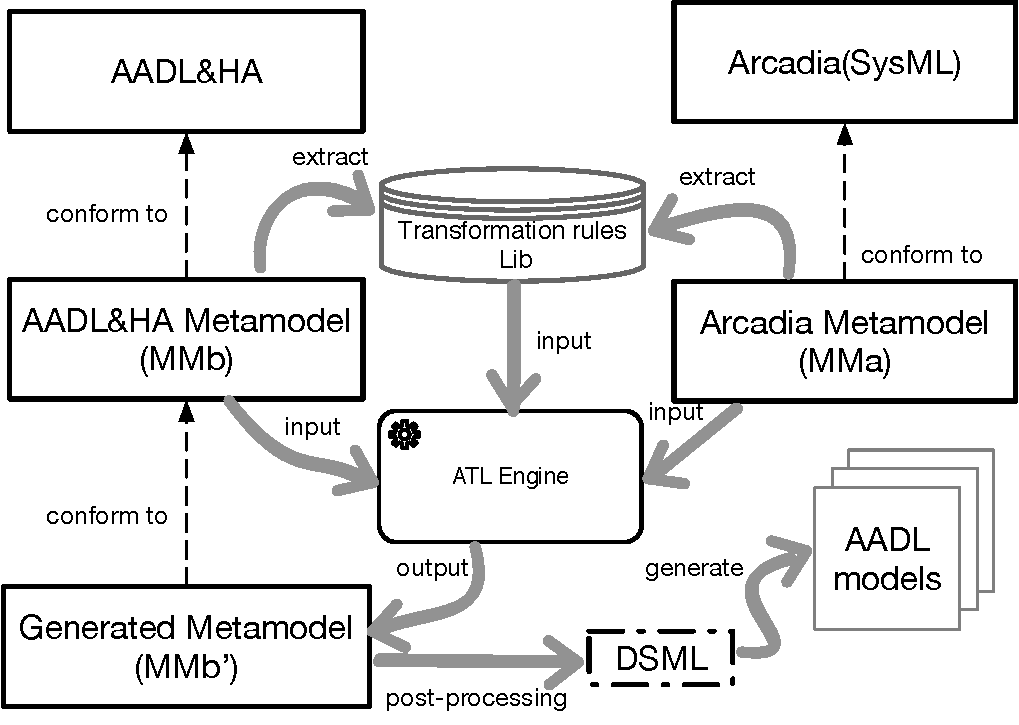
\includegraphics[width=.95\linewidth]{img/transfer_workflow}
\caption{Structure of Arcadia2AADL model transformation tools}
\label{fig:twf}
\end{figure}

Based on the translation rules defined in section \ref{sec:trans}, we implemented Arcadia2AADL transformation tool which can generate target metamodel according to original metamodels and transformation rule library. The ATL serves as a transformation engine. For more detailed information of ATL, the reader is referred to~\cite{Jouault:2006ft}\cite{Jouault:2008bz}. 
The tool architecture is shown in Fig \ref{fig:twf}. AADL\&HA (denoted as MMb) and Arcadia metamodels (denoted as MMa) are imported (input) into ATL engine and the engine is going to read transformation rules library and then the transformation engine exports (output) the corresponding metamodel (denoted as generated metamodel MMb') which is a subset of AADL\&HA, in other words, the generated metamodel is fit AADL and its hybrid annex. The generated metamodel is then further post-processed as a DSML (domain-specific modeling language) in \textit{ecore} format. Which can be used to create concrete models. Therefore, all concrete models afterward are conformed to this metamodel and will be used for further verification and analysis.  


\section{Case Study}\label{sec:imp_cs}
To show the efficacy of our approach in transforming and using produced AADL models to analyze the properties, this section presents the experimental results of analyzing the traction controlling unit of railway signaling system. By using our proposed approach, we transfer and extend Arcadia metamodel, and design AADL using OSATE2~\cite{osate2ref} with the generated metamodel. once the concrete models have been created, the scheduling property is chosen to show analysis ability through Cheddar tool. 



\subsection{Train traction controlling system (TCU)}
Train movement is the calculation of the speed and distance profiles when a train is traveling from one point to another according to the limitations imposed by the signaling system and traction equipment characteristics. As the train has to follow the track, the movement is also under the constraints of track geometry, and speed restrictions and the calculation becomes position-dependent. The subsystem of calculating the traction effective and speed restrictions is therefore critical to achieving train safe running.
Nowadays, Communication based train control (CBTC) is the main method of rail transit (both urban and high-speed train) which adopts wireless local area networks as the bidirectional train-ground communication~\cite{zhu2009train}. To increase the capacity of rail transit lines, many information-based and digital components have been applied for networking, automation and system inter-connection, including general communication technologies, sensor networks, and safety-critical embedded control system. %A large number of subsystems consisting of modern signaling systems of railways, therefore, system integration is one of the key technologies of signaling systems; it plays a significant role in maintaining the safety of the signaling system~\cite{Wang:gg}. 

This paper uses a subsystem called traction controlling system (TCU) from signalling system of high-speed railways to illustrate the model transformation from engineering level to detailed architectural level and verification of instance models. Functional modules such as calculation and synchronization will be transformed using our approach, and then non-functional properties such as timing correctness and resource correctness will be verified by simulation tool Cheddar~\cite{Singhoff:2004es}. 

The functions of the traction control system are to collect the external data by sensors such as speed sensor. The data from Balise sensors is used to determinate the track block, and then it is going to seek the speed restriction conditions by matching accurate positioning (if the track blocks are divided fine enough) and digital geometric maps data. Meanwhile, calculating speed unit received the speed data from GPS and speed control commands from HMI (Human-Machine Interface) periodically. GPS data provides speed value periodically, and HMI data send the operation command (e.g., expected speed value), then the calculating unit has to output an acceleration value and export to the locomotive mechanical system. Although they are periodic, the external data do not always arrive on time due to transmission delay or jitter. Therefore, we should use a synchronizer to make sure they are synchronized. Otherwise, the result would be wrong with asynchronous data. Similarly, to ensure the correctness of the command of acceleration (or deceleration), we applied a voting mechanism which can ensure the result is correct as much as possible. The voter must have the synchronized signal and restriction condition to dedicate to output the acceleration coefficient request to the locomotive system. The AADL diagram shown as figure \ref{fig:tcus}.     

\begin{figure*}[!h]
\centering
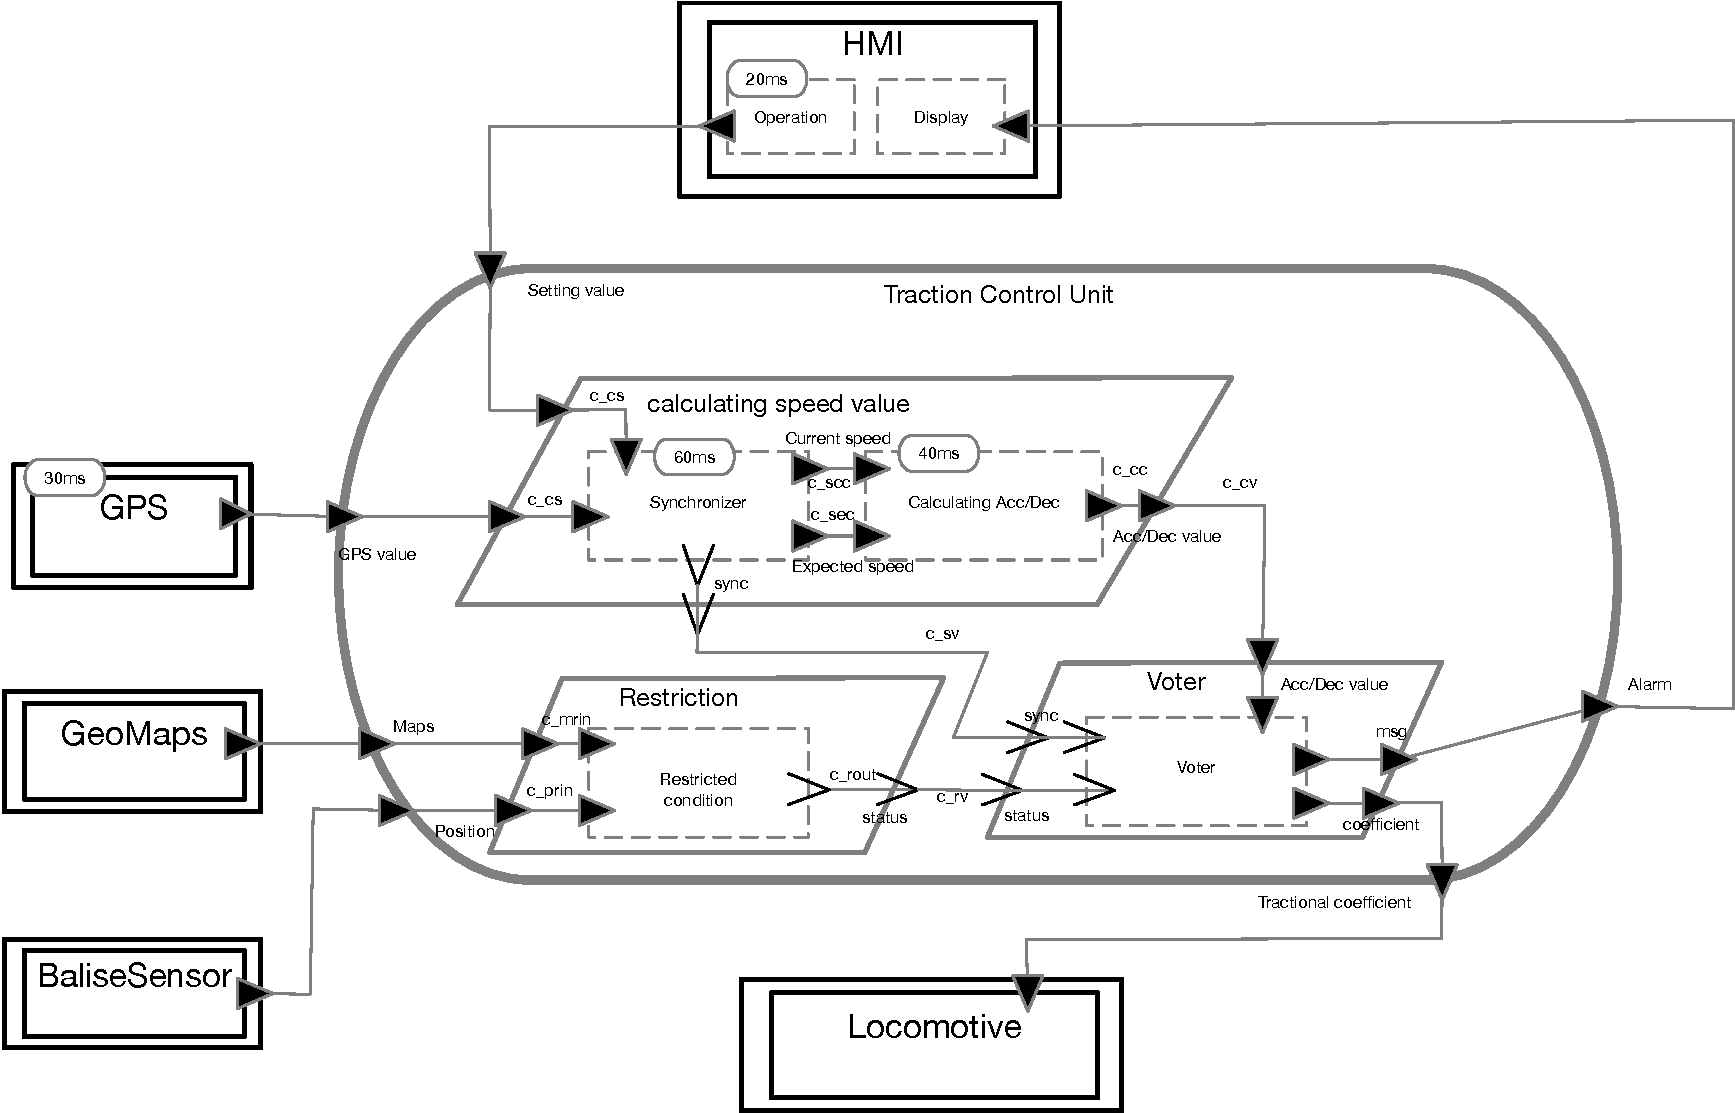
\includegraphics[width=.75\linewidth]{img/TCU_all}
\caption{AADL model for TCU of signaling system}
\label{fig:tcus}
\end{figure*}




\subsection{Model transformation}
Using the Arcadia2AADL tool, the metamodel of the TCU system in Capella is translated into the corresponding AADL metamodel with the rules and approach which describes in section \ref{sec:trans}. For instance, on the one hand, the function class is translated into the thread in AADL. To analyze the timing properties, several attributes also have been added such as protocol type, deadline, execution time, period. 

On the other hand, the physical part element Node translates to the processor in this case. Differ from simple physical Node in Arcadia; the processor element attaches rich properties such as scheduling protocol (scheduler type), process execution time. 
The allocation relationships on both physical and functional parts are translated into AADL as well.
\subsection{Schedule verification}
The external data and internal process work sequentially is an essential safety requirement of the system, and each task should be scheduled properly. However, in real-world, the risk of communication quality and rationality of scheduling must be taken into account. Therefore, the schedule verification is a way to evaluate system timing property. An Ada framework called Cheddar which provides tools to check if a real-time application meets its temporal constraints. The framework is based on the real-time scheduling theory and is mostly written for educational purposes~\cite{Singhoff:2005:SMR:1103846.1103847}.

\input{codes/cal.aadl}

Listing \ref{code:cal} shows a set of 4 periodic tasks (cal, pos, sync and setting) of TCU  respectively defined by the periods 100, 100, 40 and 30, the capacities 60, 40, 30 and 20, and the deadlines 100, 100, 40 and 30. These tasks are scheduled with a preemptive Rate Monotonic scheduler (the task with the lowest period is the task with the highest priority).
\begin{figure*}[h]
\centering
\subfigure[Schedule 1]{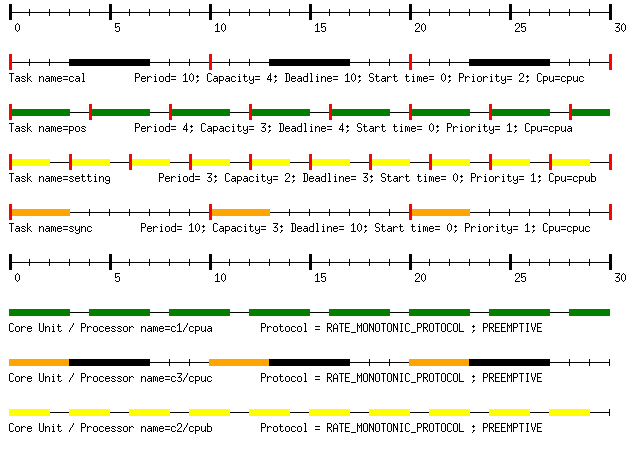
\includegraphics[width=.45\linewidth]{img/sim_left}}
\subfigure[Schedule 2]{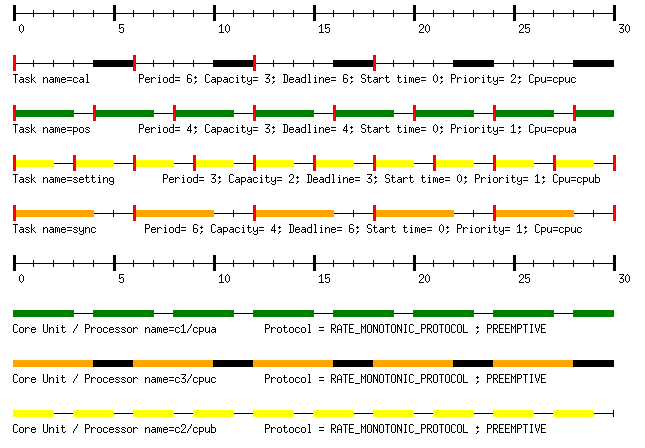
\includegraphics[width=.45\linewidth]{img/sim_right}}
\caption{Simulation results of tasks schedule}
\label{fig:sim}
\end{figure*}
For a given task set, if a scheduling simulation displayed XML results in the Cheddar. One can find the concurrency cases or idle periods (see left of figure \ref{fig:sim}, comprise the software part and physical device part). People change the parameters directly and reload simulation; an feasible solution can be applied instead. After tuning, finally, the appropriate setting has displayed as in right of figure \ref{fig:sim}. According to this simulation result, people can correct the properties value in AADL, thereby ensure the correctness of system behavior timing properties.  




%% Preamble: \pgfplotsset{width=7cm,compat=1.15} 
%\pgfplotsset{every axis/.append style={
%    font=\footnotesize,
%    thin,
%    tick style={ultra thin}},
%}
%\begin{figure}
%\begin{tikzpicture}
%    \begin{axis}[legend pos=outer north east,
%        xlabel=Time (second),
%        ylabel=Speed (km/h),
%    ]
%        \addplot+ table {codes/dataset};
%        \addplot+ table {codes/dataset1};
%        \addplot+ table {codes/dataset2};
%        \legend{caculated speed, current speed, setting speed}
%    \end{axis}
%\end{tikzpicture}
%	\caption{Train speeds}
%	\label{fig:speed}
%\end{figure}
\section{Conclusions and future work}
This paper describes a collaborative design approach between system engineering methodology Arcadia (based on SysML) and architectural design language AADL (include hybrid annex) using transformation at metamodel level. We first present a formal description of key modeling elements of Arcadia, AADL, and hybrid annex, respectively. Then translation rules from these Arcadia metamodels to AADL are formally defined. Finally, we give the implementation procedures using ATL, and a case of train traction controlling system is used to demonstrate the transformation from engineering concerned design into an architectural refinement design which can be further analyzed on scheduling properties. 
In our future work, we will study the translation rules for more elements of Arcadia and also for comprehensive SysML elements, even for others UML-like profiles such as MARTE. At the same time, we will continue to explore the AADL and its annex to support more analysis and formal verification of system design. Besides, the safety-critical systems have become a trend in industrial files. We will study the extension of AADL with verification of safety properties with transformation methodology. 



%%%%%%%%%%%%%%%%%%%%%%%%%%%%%%%%%%%%%%%%%%%%%%%%%%%%%%%%%%%%%%%%%%%%%%%%%%%%%%%%


\addtolength{\textheight}{-12cm}   % This command serves to balance the column lengths
                                  % on the last page of the document manually. It shortens
                                  % the textheight of the last page by a suitable amount.
                                  % This command does not take effect until the next page
                                  % so it should come on the page before the last. Make
                                  % sure that you do not shorten the textheight too much.

%%%%%%%%%%%%%%%%%%%%%%%%%%%%%%%%%%%%%%%%%%%%%%%%%%%%%%%%%%%%%%%%%%%%%%%%%%%%%%%%



%%%%%%%%%%%%%%%%%%%%%%%%%%%%%%%%%%%%%%%%%%%%%%%%%%%%%%%%%%%%%%%%%%%%%%%%%%%%%%%%






%\begin{thebibliography}{99}

%\end{thebibliography}
\bibliographystyle{IEEEtran}
\bibliography{bib/GENBIB}



\end{document}
